\chapter{從古典到近代量子物理}
\chapterauthor{丁安磊}
\setcounter{section}{-1}
\section{引言}
量子理論是近代的物理領域之一,量子物理的理論是非常難懂的,因為他的內容幾乎都與我們的直覺相牴觸,例如你有一定的機率可以穿牆,光波是粒子,電子是一種波,等等!不要那麼快趴下!這堂課會使用循序漸進的方式帶你探索物理的發展史,你們可以把他當作在看八點檔,時不時的會出現超展開的情節,請想像你就是那些科學家,跟隨著他們的腳步探索物理。(以下的歷史不保證完全正確)

如果以下的數學讓你感到頭昏,你可以忽略它,這不會影響到你的體驗,但有件事你必須謹記在心:數學公式與推導在物理學是不可或缺的,他展現了物理學的美妙和邏輯,因為數學能以最客觀和最精密的方式描述物理定律。

還有,科普與科研是完全不同的,科學雖然只能被少部分人研究,但科學能被大部分人欣賞,不能被大部分人欣賞的科學通常是沒有被研究好的科學。

現在讓我們進入時光機,回到西元前的時代,你現在在古希臘,辯士學派杜絕探究世界的真理,但希臘三大哲學家之一亞里斯多德思考著他的自然哲學。
\section{古希臘物理學(亞里斯多德物理學)}
從西元前300年左右,最早的物理學由古希臘哲學家亞里斯多德開創,由於亞里斯多德的地位,這些理論維持了將近兩千年都沒有被質疑,雖然它作為物理學的開端,但對於現在的我們來說,裡面有些理論看起來都很智障,舉幾個例子如下:
\begin{itemize}
\item \textbf{四元素理論}:亞里斯多德認為四種主要元素組成地球:土、氣、水及火,相信這個大家都聽過,對於現在的我們來說當然很唬爛。
\item \textbf{地球是宇宙的中心}:亞里斯多德認為宇宙萬物都繞著地球轉,從地球上看,不管是太陽、月亮、恆星,看起來都是繞著我們轉的。
\item \textbf{物體受力會做直線運動}:這對於沒學過\textbf{牛頓力學}的人來說看起來很合理?不過很遺憾,他是錯的。
\item \textbf{光線是從人的眼睛射出}:這顯然是錯的,它們可能是覺得夜晚中貓咪的眼睛會發光,所以這麼認為,不過貓咪很可愛這次我就原諒你吧。
\end{itemize}
亞里斯多德對於物理學的理解加上他的權威,建立起了看似屹立不搖的大樓,兩千年內沒有人能推倒這棟大樓,塑造了中世紀的學術思想,但直到牛頓這個叛亂份子居然輕鬆地用他的牛頓力學推倒了這棟大樓,並建立起了牛頓的經典力學體系,我們來看看這棟大樓的豆腐渣工程在哪:亞里斯多德雖然嘗試以理性來解釋大自然,但這些理論和現代科學比較起來,都有以下共通點:過於主觀、缺乏嚴謹證明。但我們還是要感謝亞里斯多德先生,作為先驅,你盡力了。

現在直接飛到牛頓那邊,來看看他做了什麼吧。


\section{古典物理學}
從中世紀開始的科學革命,帶給了科學突破性的進步,其中的\textbf{科學方法}的變革,帶給了引導著各門科學的發展,其中當然也包含物理學,物理學在這個時期逐漸壯大、統一,每個領域都逐漸的變成神聖而不可分割的一部分。注意,以下的理論是並立發展的,不是依照先後順序排列的。 
\section{古典物理學-牛頓力學}
牛頓寫了一本書《自然哲學的數學原理》,裡面使用嚴謹的數學來描述力學定律,他把物體的運動模式統合成三條牛頓運動定律。還有被蘋果砸到之後想到的萬有引力定律,表示兩物體之間的引力與他們的質量成正比,與他們之間的距離平方成反比。
\begin{figure}[H]
\centering
\graphicspath{{physics/}}
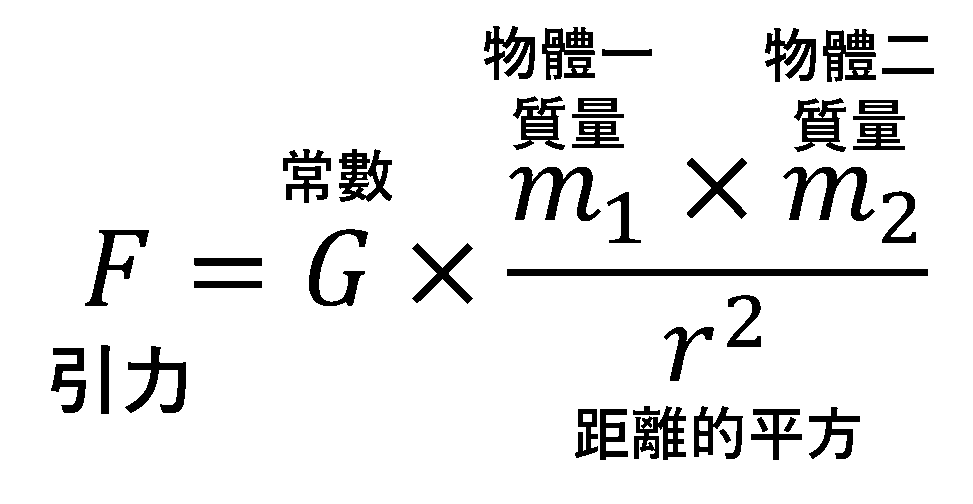
\includegraphics[width=5cm, center]{newton-law.png}
\caption{牛頓的萬有引力定律}
\label{fig:newton-law}
\end{figure}

\section{古典物理學-電磁學}
電學的方面,庫倫使用扭秤實驗得到了兩個帶電物體之間的電力
\begin{figure}[H]
\centering
\graphicspath{{physics/}}
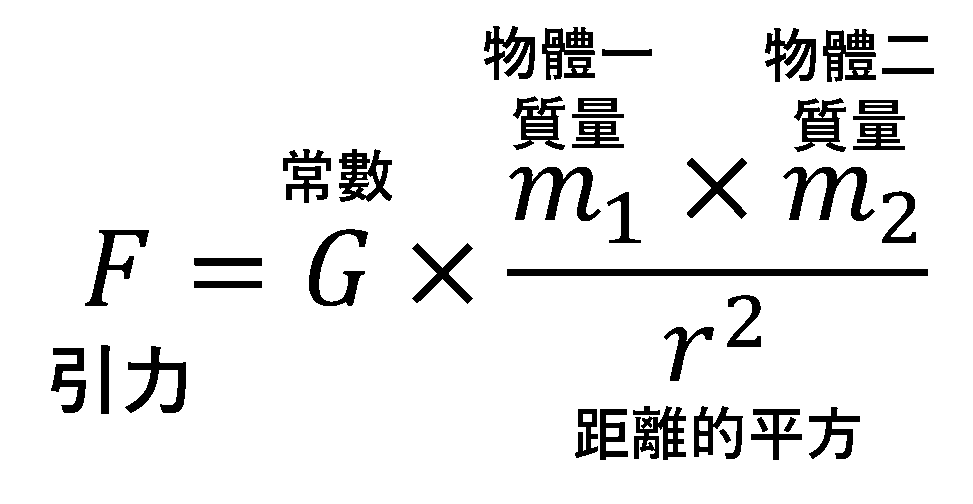
\includegraphics[width=5cm, center]{newton-law.png}
\caption{庫侖定律}
\label{fig:coulomb-law}
\end{figure}
有沒有覺得眼熟?他的形式就和重力的公式一樣!\\
磁力的形式比較複雜,但我們也能發現距離平方反比的特性
$$\Updelta B \propto \frac{I \Updelta L}{r^{2}}\mbox{;}F=q v B $$
\begingroup
\captionof{figure}{磁場的性質和磁力與磁場的關係(沒有解釋方向)}
\endgroup
\begin{tcolorbox}[breakable, title={專欄:平方反比定律}, before upper={\parindent2em}, parbox=false]

牛頓重力公式和庫倫定律都具有一樣的形式,我們可以發現他們的共同性質就是,力與距離的平方成反比,這是巧合嗎?我不這麼認為。我們以光線為例子來說明平方反比定律,假設杰穎想要拍一個燈泡(光源),他為了不讓照片曝光太亮或太暗,要如何調整光圈的大小?(光圈可以調整相機接受光線的面積大小)

我們可以將光想成許多條的光線平均向外擴散,我們假設光線不會因為傳播而變弱,所以如果我們在以光源為圓心的球殼上,不論半徑多大,接受到的光線數目是一樣多的。
\begin{figure}[H]
\centering
\graphicspath{{physics/}}
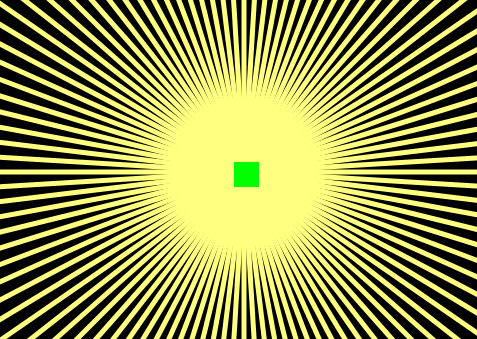
\includegraphics[width=5cm, center]{light.png}
\caption{光線散播圖}
\label{fig:light}
\end{figure}
當杰穎距離光源越遠,雖然光線一樣多,但他可以接收到的\textbf{光線密度}就會越小,也就是說,杰穎的光圈就需要張的更大,來接收足夠多的光線,下圖展示光圈的大小與距離的關係。
\begin{figure}[H]
\centering
\graphicspath{{physics/}}
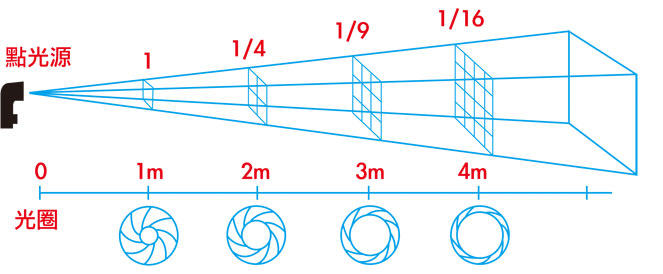
\includegraphics[width=7.5cm, center]{square-light.png}
\caption{平方反比定律的直觀理解}
\label{fig:light}
\end{figure}
在物理上,光線的密度定義為\textbf{照度},光線強度定義為\textbf{亮度},表示式為:
$$ \mbox{照度} = \frac{\mbox{亮度}}{r^2} $$

那麼,在力的部分,我們要如何思考平方反比定律呢?

我們引入力場的概念,重力場的大小定義如下,同樣與距離平方成反比,電力場擁有相同的情況

$$ \mbox{重力場 } g = \frac{GM}{r^2} \mbox{;電力場 }E=\frac{kQ}{r^2} $$

這裡以重力場為例,$M$代表建立這個場的質量的值,當有質量為$m$的物體位在這個場內,會施給他大小為場強$\times m$的重力,你可能會想說,為什麼我們要特地定義出一個場?原本的公式不是就可以描述重力的大小了嗎?

最初,會定義場的概念,是為了解釋\textbf{超距力}的作用,請思考一個問題,如果太陽瞬間消失了,地球會馬上飛出去嗎?答案是不會,我們必須考慮重力場傳播的速度,這個速度\textbf{就是光速},所以說,當太陽瞬間消失,等到過了8.3分鐘,地球將變為一片黑暗,並同時脫離軌道(因為太陽與地球的距離為1億5千萬公里,光速為每秒跑30萬公里,所以光與重力場從太陽傳播到地球的時間約為8.3分鐘),和光線密度一樣,我們可以把力場當成\textbf{力線密度},這也很好的解釋為什麼重力場會滿足平方反比定律。

電場的情況較複雜一些,因為電場的變化會產生磁場,反之亦然,以下將討論電場與磁場的關係。
\end{tcolorbox}

一開始,大家都覺得電與磁之間沒有關係,有人專門研究電學,有人專門研究磁學,直到一位大學教授厄斯特出於好奇心,將指南針放在流通著電流的線上,結果發現指南針的指針偏轉了!

接著,有許多人在研究電場與磁場之間的關係,如安培、法拉第等人,但最後被馬克士威統合成美妙的四條方程式。

$$ \nabla \cdot \mathbf{E}=\frac{\rho}{\varepsilon_{0}} $$
$$ \nabla \cdot \mathbf{B}=0 $$
$$ \nabla \times \mathbf{E}=-\frac{\partial \mathbf{B}}{\partial t} $$
$$ \nabla \times \mathbf{B}=\mu_{0} \mathbf{J}+\mu_{0} \varepsilon_{0} \frac{\partial \mathbf{E}}{\partial t} $$

\begingroup
\captionof{figure}{馬克士威電磁定律}
\endgroup

這四條方程式稱為馬克示威方程組【參閱附錄:\autoref{maxwell}】,我先給這方程組下一個評語:困難又簡單,難就難在他用了複雜的數學描述,簡單就簡單在他只用四條方程就描述了\textbf{大部分}電與磁的特性與關聯(注意是\textbf{大部分}) \par

你可能會想問,這是甚麼鬼?三角形是啥?為什麼那個長得像6的東西不能消掉?不用擔心,你不用懂這些計算,我只告訴你這些方程式告訴我們的結論:

\begin{itemize}
\item 第一條:其實他就是庫倫定律,只是物理學家喜歡把他寫成看起來一樣而且很酷的樣子,呵呵。
\item 第二條:它表示世界上不存在磁單極,甚麼意思?就是說我們不能只有N極和S極單獨存在,N極和S極一定會並存,不像電荷能夠有分開的正電荷和負電荷單獨存在,如果你把一個磁鐵分開,他會變成兩個磁鐵。
\item 第三條:他表示如果磁場發生變化,就會產生電場
\item 第四條:他表示如果電場發生變化、或有電流,就會產生磁場。
\end{itemize}

\begin{figure}[H]
\centering
\graphicspath{{physics/}}
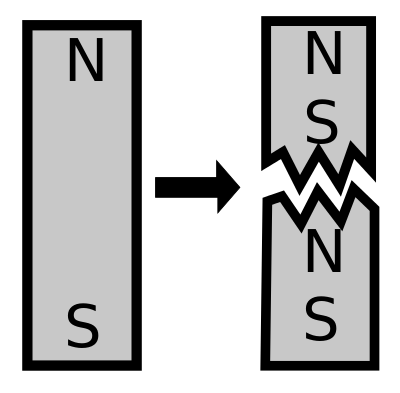
\includegraphics[width=5cm, center]{mag.png}
\caption{磁鐵分開後會變兩個磁鐵}
\label{fig:mag}
\end{figure}

當然,以上這些說法都是簡略到不能再簡略,要想真正搞懂你需要先學會向量、微積分、向量微積分(這東西和微積分簡直是天差地遠),如果你對這種困難的數學有興趣的話,請參閱附錄,也歡迎\textbf{來考武陵並加入物理讀書會(偷偷業配)}

如果你覺得沒興趣那也沒差,把結論收在心裡,我們繼續我們的旅程。

馬克士威利用他的電磁理論推論出\textbf{電磁波}的存在,細節推導很困難,不過你們可以這樣理解(雖然有點唬爛),第三條和第四條分別說電會生磁,磁會生電,所以如果當其中一個開始變化,就有可能會一直互相產生,並且他們震盪的\textbf{頻率決定這個電磁波在我們眼裡的顏色!}
\begin{figure}[H]
\centering
\graphicspath{{physics/}}
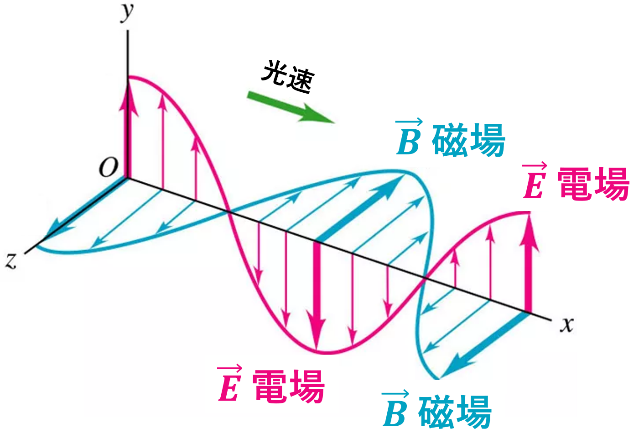
\includegraphics[width=7.5cm, center]{mag-wave.png}
\label{fig:mag-wave}
\end{figure}
二十多年後,赫茲在做放電實驗時,偶然發現身邊的一個線圈兩端發出電火花,原來是一個個小火花在迅速地來回跳躍。赫茲想到,這可能與電磁波有關。

後來,赫茲製作了一個十分簡單而又非常有效的電磁波探測器,這個探測器可以檢驗電磁波,赫茲把這個探測器放到電容旁邊,當電容的電壓足夠高,就會導通空氣,產生電火花,所以應該會產生電磁波,赫茲用諧振環接收電容產生的電磁波,諧振環中發出了電火花。所以,諧振環就好像收音機一樣,它是電磁波的接收器。就這樣,人們懷疑並期待已久的馬克士威電磁波理論終於被實驗證明了,此時風平浪靜的物理學貌似達到了巔峰,但他不知道這個實驗是個雙面刃,將帶給物理學一場腥風血雨的改革。

赫茲做實驗的時候,因為接收器的火花很小,幾乎看不到,他為了觀察清楚,把實驗室的燈關掉,而旁邊的發射器不斷的打出火花,也會對觀測接收器造成影響,於是他就找了一個塑膠箱子(塑膠1850年就被發明了),把他的接收器蓋住,然後在上面挖一個小洞,從小洞裡看接收器,或許這樣就能夠看得更清楚了吧?結果是,並沒有,用塑膠箱子蓋住之後,從接收器上看到的火花反而變得更微弱了。而且他還發現,如果拿高頻段的光例如紫光、紫外光,照著接收器,電火花會更容易出現。這個發現赫茲沒有做太多思考,但他不知道,他剛剛給繁榮的電磁理論埋下了一個伏筆,可惜的是,他在三十多歲的時候就過世了,無法看到接下來物理學的風起雲湧。
	
\section{古典物理學-熱力學}
熱力學研究溫度、壓力、體積、熱量、內能、熵等等物理量的關聯,你可以粗暴的把他當成研究熱的學科,這裡不多做贅述,就和竣程的化學課有點類似?
\section{古典物理學-光學}
終於要開始最有趣的部分了,光學的發展史可以比喻成物理大陸上最一場激烈的戰爭,持不同觀點的人們爭論著:光究竟是波還是粒子?我們再回去找這場戰爭的導火線:牛頓。

這裡插播一句話:人們總是傾向於巴著自己最了解的事物不放,因為已耗盡一生傾注全心全意於這些事物,不願放棄自己所堅信的事物,卻也失去了甚麼。請把這句話放在心裡,因為在物理學的發展上,這個情況不斷的出現。

心靈雞湯喝完,回到正題,時光機來到牛頓的小房間裡,這裡一片漆黑,忽然,一束白色光線打進來,散播成七種顏色的光,在屋內的牆壁上,出現了一條長長的彩色寬帶,牛頓看到了太陽的光能夠分散成七種顏色,於是他認為白光是七種顏色的光粒子的混合,三稜鏡會將這七種顏色的粒子分開,他把他的研究成果交給英國皇家學院的一個三人的評議會。

三人中的一個人,名叫虎克,對,就是那個玩彈簧的虎克,也是那個觀察到細胞的虎克,虎克認為光是一種波,他是光波動學派的大將之一,光波動學派的創始人叫做格里馬第,格里馬第發現了光的繞射現象,我們知道水波也會發生繞射,所以他合理的推斷光會是一種波,虎克受到格里馬第的影響,他認為光是一種類似於彈簧波的縱波,所以當他看到牛頓的研究成果時,虎克對他的觀點做了非常嚴厲的批評,這下不得了,虎克顯然是沒有達爾的探測鏡,他不知道自己眼前的這個牛頓,戰鬥力超過9000!牛頓從沒見過有人這樣批評他,馬上爆氣花四個月寫出一篇長文砲轟虎克,虎克被嚇得暫時收斂,這場第一次波粒戰爭就此結束。

等等!還沒結束,這時,惠更斯加入了戰局,他在歐洲大陸上全力發展光的波動說,繼承了虎克的思想,引入了波前的概念,他用了自己的理論推導出了光波的反射和折射定律,後來甚至能夠拿來解釋方解石(某種碳酸鈣的結構)的雙折射現象,甚至是自己的對手牛頓發現的牛頓環現象,也被惠更斯的理論所解釋。不過很遺憾,惠更斯帶給光波動學派的興盛是暫時的,你眼睛業障重,因為牛頓站在波動學派的後面,他非常火,牛頓對虎克的仇恨久久無法散去,只要英國皇家學會有虎克的存在他就絕不踏進那裡一步。

等到惠更斯、虎克相繼過世,牛頓當選為英國皇家學會的主席,這時候的牛頓已經不是當年的那個牛頓了,他現在是寫了《自然哲學的數學原理》的牛頓,發明了微積分的牛頓,身為國會議員、造幣局局長的牛頓,牛主席在光粒人民共和國稱帝的第一步已經開始,他出版的《光學》用粒子說證明了色彩疊合、分散、薄膜透光、牛頓環、繞射、雙折射(細節不多做贅述),對光波動學派造成可觀的打擊,波動學派沒有了他們的領袖,它們自己內部也沒有個完善的理論,\sout{經常在立法院打架},終究難逃被統一的命運,終於,一道光線,各自表述的呈現了一面倒的情況,第一次波粒戰爭,由光粒子學派勝利。

轉瞬之間,一個世紀過去了,光粒子的觀念烙印於人們的思想中,但在這時,英國出現了一位甚麼都會的全才,叫做楊(Young),不是很年輕的那個Young喔,有些人也就叫他楊格包括我,這時你的英文老師可能會爆氣,因為ng裡面的g不發音,她會請你去把一篇作文重寫七次。總之,這個楊格呢是個甚麼都會的人,就像我們班的電神杰穎(編按:並沒有),什麼都知道,楊格被譽為「世界上最後一個什麼都知道的人」,他在13歲時,已經會說希臘文、拉丁文、希伯來文、義大利文與法文,楊格後來成為了一位醫生,楊格遇到的病人中,許多人都在跟他抱怨視力逐漸模糊的問題,那個時候近視的人就等於全盲了,於是楊格開始了他對光學的研究,想要治療這些人,最初,楊格研究牛頓環現象時,發現這種明暗相間的條紋可以用波的干涉來解釋,他也用他的干涉理論證明出了繞射的現象,也設計了一個非常經典的實驗來加強他的理論-光的雙狹縫干涉實驗。
	
	這個實驗的方法是,在面板後面放一個點光源,並且在面板上鑽出兩個非常狹窄的縫隙(雙狹縫),並觀察面板前面的牆壁上的亮度,如果牛頓的粒子說是對的,實驗的結果可能會是中間最亮,而越遠離中間則越暗【如圖\ref{fig:exp1}】,但楊格做出來的結果【如圖\ref{fig:exp2}】所示,產生了和水波一樣的干涉條紋!但這時候大家都沉浸在牛頓的美好世界裡,楊格的論文無處發表,他只好把他印成小冊子在路邊兜售,結果也只賣出一本。

\begin{figure}[H]
\centering
\begin{minipage}{0.5\textwidth}
\graphicspath{{physics/}}
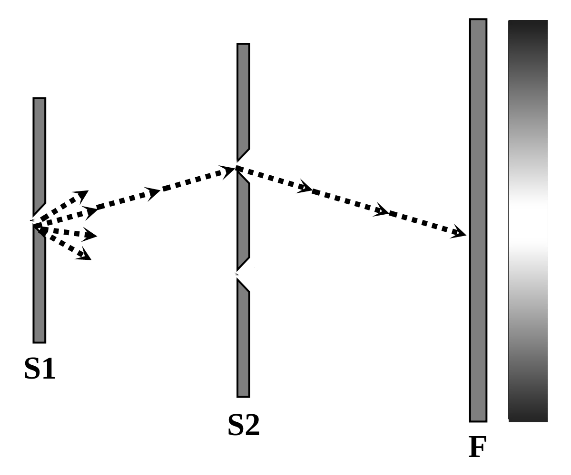
\includegraphics[width=\linewidth, center]{exp1.png}
\caption{粒子說預測的結果}
\label{fig:exp1}
\end{minipage}%
\begin{minipage}{0.5\textwidth}
\centering
\graphicspath{{physics/}}
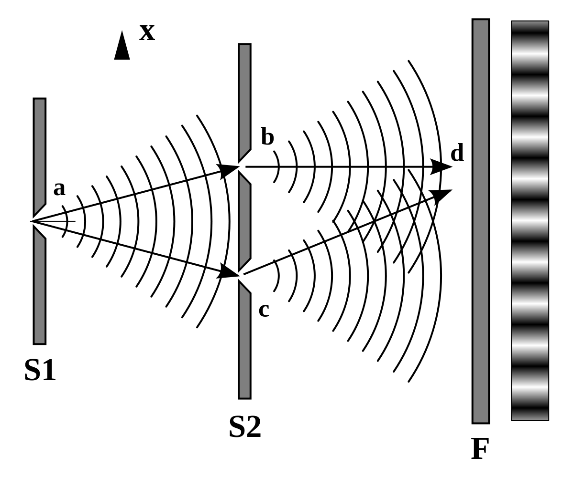
\includegraphics[width=\linewidth, center]{exp2.png}
\caption{楊格的實驗結果}
\label{fig:exp2}
\end{minipage}
\end{figure}

但是微粒派馬上開始發現,這次的對手實力不容小覷!微粒說無力反駁楊格的實驗結果,因為不管光粒子怎樣飛,都不會有兩個粒子碰在一起變暗的情況發生,微粒說為了反駁,派出了馬呂思,他使用技能「光的偏振現象」!這時光的波動說無法解釋他所發現的光偏振現象,第二次波粒戰爭開打,戰況又陷入膠著。

決勝時刻到來了,法國科學院(簡稱法科),公布了一道懸賞題目,內容是用精密的實驗與理論來確定光的繞射現象,法科的許多評委都是支持微粒說的人,他們的本意可能是希望有人能夠用微粒說來說明光的繞射。這時有個耍白目的人提交了一篇論文,他叫做菲涅爾,他使用光的波動觀點嚴密的推導出了光的繞射問題,他的推導過程天衣無縫,(你可能會問說,楊格不是已經用波動推導過繞射了嗎?很遺憾,根本沒人知道,包括菲涅爾。)但是法科的評委之一-帕松,發現菲涅爾的理論應用在圓盤的繞射上的時候,會在圓盤的中心出現一個亮點!你拿光照一個圓盤,中心會出現一個亮點?帕松覺得這真是笑死人了,帕松給了菲涅爾的理論一巴掌,但是法科的評委之一,阿拉果,又帶給波動派一個超展開,他堅持要給帕松發現的亮班做一個實驗,帕松本人則認為這個現象荒謬至極到不必做實驗來驗證,就在帕松認為自己又一次帶領微粒派擊退波動派的同時,阿拉果照出了那個亮點!戰況大逆轉!菲涅爾的理論大獲全勝,而最搞笑的事,這個圓盤繞射產生的亮斑明明是帕松否認的現象,結果被命名為帕松亮斑,真是物理史上的一大羞辱。

\begin{figure}[H]
\centering
\graphicspath{{physics/}}
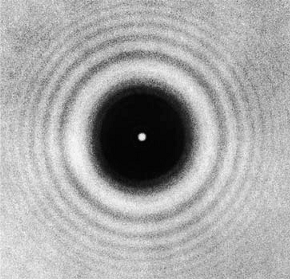
\includegraphics[width=7.5cm, center]{arago.png}
\caption{帕松亮斑}
\label{fig:mag}
\end{figure}

其後波動學派對於粒子學派的反攻毫不留情。第一波進攻,為了解決馬呂斯的偏振問題,菲涅爾假設光是一種橫波,而不是他們以前認為的那種縱波,被打敗的馬呂斯只好回到他的悲慘世界(沒人懂梗好嗎)。

再來,第二波進攻,說到這裡,我們來回憶一下牛頓是如何證明光的折射定律的,當光線從低密度的介質進入到高密度的介質,比如說從空氣進入到水或是玻璃好了,牛頓認為當光線在空氣中運行時,因為四周的萬有引力都一樣,所以光線會直線前進,但是當光運行到空氣與水之間時,一邊是空氣的萬有引力,一邊是水的萬有引力,因為水的密度更高,所以水的萬有引力比空氣更強,於是造成光在空氣與水之間被往水的方向拉動,所以對於粒子說而言,因為跑到水裡會被拉一下,光在水中的速度應該要更快才對。

第二波進攻是傅科和斐索的實驗,這時候科學的技術已經能夠測量光速了,於是他們著手測量光在空氣與水中運行的速度,這個實驗結果一旦出來,就決定了最終的勝利,結果出來了!光速在水中運行的速度只有空氣中速度的四分之三!光速在水中運行的速度只有空氣中速度的四分之三!

第三波進攻帶領波動的軍隊迎向完全的勝利,這次軍隊的將領-馬克士威,使用他的理論預測出電磁波的存在,並且計算出電磁波的速度,就等於光速!波動派終於反攻大陸,波動主義,統一光學,讓稱帝了一百多年的牛頓理論下台。

\section{黑體輻射}
不論是科普教材,還是大學課本,要介紹量子物理時都會提到黑體輻射,其實黑體輻射這個概念聽起來好像很難,但其實他就在你我身邊,因為只要溫度高於絕對零度,物質的粒子就一定會有震盪,根據馬克士威的電磁學理論,只要帶電粒子加速就會產生輻射,如果你聽不懂,你只要知道所有物體都會產生輻射電磁波就對了。
\begin{tcolorbox}[breakable, title={專欄:輻射函數圖}, before upper={\parindent2em}, parbox=false]

所有物體都會輻射?那為什麼我們看不到呢?因為溫度太低的物理的輻射都是紅外線,像是人體(37°C)輻射出的電磁波是紅外線,肉眼是看不到的,但當溫度逐漸升高,像是燒紅的木炭、鐵塊等等,因為粒子震動變得更厲害了,導致輻射出的電磁波頻率越大。某些物質甚至可以燒到變藍色、紫色、甚至到散發出紫外線!

我們知道,物體會輻射出電磁波,但因為物體內的帶電粒子不一定會有相同的震動頻率,所以這個物體內的帶電粒子可能會有各種的震動頻率,進而導致物體發出的電磁波也會有各種頻率的喔。右圖中的許多曲線代表不同溫度所輻射出的各種頻率電磁波的強度,如果還是覺得不太理解,先嘗試關注其中一條曲線,像是T=4000(T是溫度),我們可以發現在這個溫度下,物體輻射出最多的電磁波頻率在紅外線的部分,而在T=8000最多的是黃綠色的光(雖然你們看不到)

\begin{figure}[H]
\centering
\graphicspath{{physics/}}
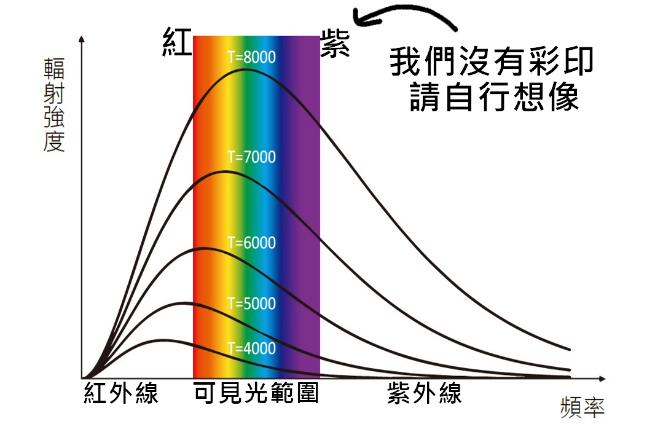
\includegraphics[width=7.5cm, center]{radiation.png}
\label{fig:rad}
\end{figure}
\end{tcolorbox}

黑體(Blackbody)是甚麼?我們知道物體會吸收、反射、輻射光線,黑體是一個物理學家想像出來的物體,我們稱為理想黑體,物理學家就是這麼任性,他只會吸收、輻射光線,而不會反射,但現實世界其實還是有能夠近似理想黑體的東西,例如太陽就很逼近一個理想黑體,你可能想說太陽明明一點都不黑啊?嗯…其實物理學家取名字也很任性。

古典物理學的研究過程大致如下:(1)發現某個現象(2)做實驗找出這個現象的數據(3)研究理論並推導出與實驗數據相符的結果。好了,現在你有一個黑體的模型了,他不會反射,就是這麼簡單,物理學家開始做實驗,找出黑體輻射的函數圖(上面那個),接著進到最後一步,使用各種理論推導出實驗的結果!首先第一位上場的是維恩,奮筆疾書,揮舞著他的鋼筆,使用寫出了維恩公式,把它的函數圖畫到紙上,高頻段的曲線和實驗數據很符合!但眼神往圖紙的左方一撇,低頻段的曲線居然與實驗數據有偏差!這不可能!一定是實驗誤差!但很遺憾,實驗是準確的,不管做幾次,曲線都長那樣。

後來有一個人叫做瑞立,他也來參與推導黑體輻射公式的工作,京士也來幫忙,他使用能量均分定理,推出了瑞立-京士公式。嗯,很棒,低頻段的曲線跟實驗數據一模一樣,但相似的場景再次上演,眼神往圖紙的右方一撇,居然飛出去了!這是不可能的!這代表物體會輻射出無限大的高頻率電磁波!這被稱為紫外災變,意思是輻射在紫外線頻段放出的巨大能量。
\begin{figure}[H]
\centering
\graphicspath{{physics/}}
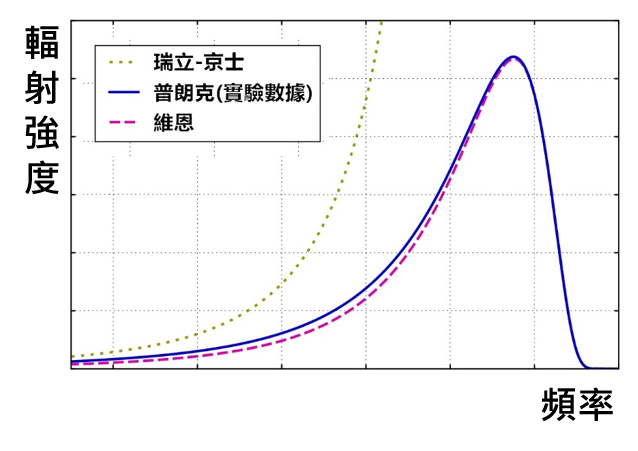
\includegraphics[width=5cm, center]{ultraviolet-catastrophe.png}
\label{fig:ultraviolet-catastrophe}
\end{figure}
其實在維恩推出他的公式之後,一位科學家普朗克也來對黑體輻射公式進行推導,他發現一項驚人的事實,他改變維恩的假設,加入「能量不連續」的假設,居然推出了和實驗數據一模一樣的數據!但這個「能量不連續」是什麼意思?他代表物體放出的輻射能量不是連續的,會有一個最小單位的能量,稱為\textbf{能量子}(energy quanta),而且這個最小單位的能量還正比於輻射電磁波的頻率,我這裡我寫下影響整個量子物理的公式。
$$E_{\mbox{最小單位}} = hf$$
直接這樣講感覺有點難懂,我們來做一些比喻,假設電磁波要把輻射能量帶出去的,把電磁波想像成攜帶能量包的人,但他每次只能拿幾包而已,沒有人再拿半包或0.9487包的,這稱為\textbf{能量量子化}。

\section{光電效應}
幾年後,愛因斯坦一邊發表狹義相對論,一邊研究光電效應問題,什麼是光電效應,還記得赫茲當年做得實驗嗎?如果有高頻率的光在照著發射器,更容易被打出電火花。其後有許多科學家投入相關的實驗,這些人的研究有一個結論,如果在乾淨的鋅金屬的表面(沒有會隔絕鋅金屬的氧化鋅),拿紫外線或紫光持續照射,會變成帶正電荷,合理推斷是表面帶負電的電子飛走了;但是如果拿紅外線或紅光照,不管拿多強的光,或是照多久的光,他都不會帶正電荷。

觀察敏銳的同學可能已經發現了,光電效應和古典電磁學是不協調的!為什麼?

電磁學認為,光是一種電磁波,他的強度(振幅)代表了他的能量,如果增強強度或增加照射的時間應該能夠打出更多、更高能量的電子。不過光電效應卻表明,只要你的電磁波頻率低於某個低限頻率,是無法打出任何電子的,但當頻率高於這個\textbf{低限頻率},隨便打都能打出電子,並且如果在這時候把強度增加,每個電子飛出來所帶有的動能,都是一樣的,只是飛出來的電子數增多了而已。

愛因斯坦也同樣受到這個問題的苦惱,他思考著:「提高頻率才能打出電子,……,提高頻率,提高頻率,提高頻率!?」他靈光一閃,燈泡忽然出現在他的頭上,他想到了普朗克的能量子,「嗯…,按照普朗克的說法,光的能量在空間中應該也不是連續的吧,而是由一些數目的能量子所組成的,好!就叫他光量子吧!」

後人把愛因斯坦的光量子(light quanta)稱作光子(photon)。

從愛因斯坦假設的光量子出發,一切都變簡單了,頻率更高的光線比如紫光、紫外光,根據普朗克的理論,會擁有更大的能量,因此當紫外光子作用到金屬表面時,就能激發出更高動能的電子,但是低頻的光,他的光子的能量太低了,沒辦法把電子激發出去,有些人可能會有問題:那為什麼不能讓很多的光子合作打出一個電子呢?這裡有個不太精確的解釋,但能夠說服你,當第一個光子將電子激發,一旦他沒有完全脫離,他會在非常短的瞬間掉回去,所以第二個前來的光子無法和第一個合作。

\begin{figure}[H]
\centering
\graphicspath{{physics/}}
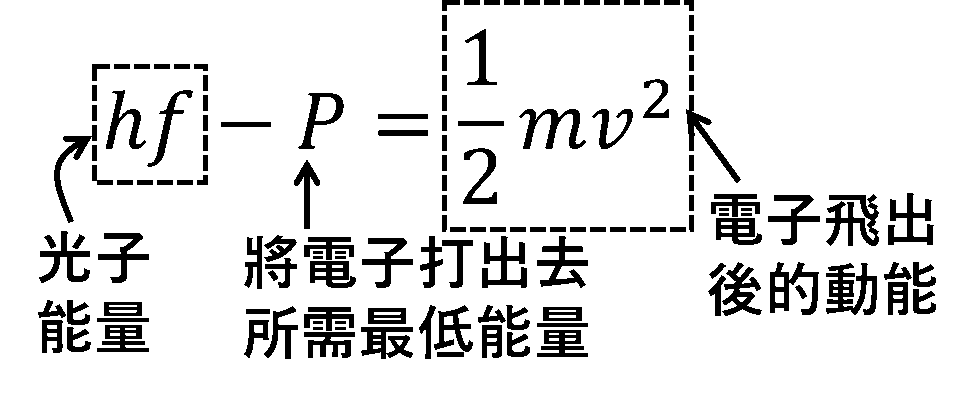
\includegraphics[width=5cm, center]{photon.png}
\label{fig:photon}
\end{figure}

這裡引用《量子物理史話》裡面的解釋(不瞞你說,前面蠻多也是參考來的)

{\Kai 我們把光電效應想像成一場有著高昂入場費的拍賣。每個光子是一個顧客,它所攜帶的能量相當於一個人擁有的資金。要進入拍賣現場,每個人必須先繳納一定數量的入場費,而在會場內,一個人只能買一件物品。}

{\Kai 一個光量子打擊到金屬表面的時候,如果它帶的錢足夠(能量足夠高),它便有資格進入拍賣現場(能夠打擊出電子來)。至於它能夠買到多好的物品(激發出多高能量的電子),那要取決於它付了入場費後還剩下多少錢(剩餘多少能量)。頻率越高,代表了一個人的錢越多,像紫外線這樣的大款,可以在輕易付清入場費後還買的起非常貴的貨物,而頻率低一點的光線就沒那麼闊綽了。}

{\Kai 但是,一個人有多少資金,這和一個“代表團”能夠買到多少物品是沒有關係的。能夠買到多少數量的東西,這只和“代表團”的人數有關係(光的強度),而和每一個人有多少錢(光的頻率)沒關係。如果我有一個500人的代表團,每個人都有足夠的錢入場,那麼我就能買到500樣貨品回來,而你一個人再有錢,你也只能買一樣東西(因為一個人只能買一樣物品,規矩就是這樣的)。至於買到的東西有多好,那是另一回事情。話又說回來,假如你一個代表團裡每個人的錢太少,以致付不起入場費,那哪怕你人數再多,也是一樣東西都買不到的,因為規矩是你只能以個人的身份入場,沒有連續性和積累性,大家的錢不能湊在一起用。}
\section{原子結構}
說完了黑體輻射與光電效應,來說說古典物理碰到的另一個問題:原子的結構。因為這在國二理化是一個章節,這裡為了節省篇幅,就不講得太細了。

科學家們所提出的原子模型發展如下。
\begin{enumerate}
\item \textbf{道爾頓原子模型}:道爾頓認為物體的最小基本單位是原子,無法再細分
\item \textbf{湯木生葡萄乾布丁模型}:J.J.湯木生發現了電子,但原子是電中性的,所以他認為原子內是數量一樣的電子和不知道是甚麼的正電荷鑲嵌在一起而成,他覺得整個原子可能有一個大區域的正電荷布丁,幾個電子在上面跑,看起來葡萄乾(?)
\item \textbf{拉塞福行星軌道模型}:因為他的α粒子散射實驗,他認為正電荷是集中在中心的小區域內,稱為原子核,電子以一個軌道繞著原子核運轉,就像行星繞著恆星轉一般。
\end{enumerate}
國中有講的原子模型大概就這三個,後面什麼中子之類的東西我就不多討論了,但其實原子模型的發展還沒有結束,為什麼,因為拉塞福的模型有個致命的錯誤,根據馬克士威的電磁理論,當電子運行在軌道上做等速圓周運動,就必定有個向心加速度,有加速度就會輻射出能量,那這樣電子就會不斷耗散能量直到墜落到原子核!個屁啦!怎可能,以上這些如果是真的將會在不到一秒鐘內發生,但我們現在還不是活的好好的,所以這個模型一定是錯的……嗎?

好了,先平復一下情緒,跟著拉塞福的學生-波耳一起來想這個問題。

有一天拉塞福要求波耳幫忙思考這個理論的穩定性問題,波耳思考著:「對於這個問題來說,要嘛老師的行星模型是錯的,要嘛馬克士威的電磁理論是錯的,只能二擇一」
	
「不管馬克士威的電磁理論有多麼的簡潔美妙,現在沒有人真正的驗證在原子的微觀尺度的電磁理論是否正確,我寧可拋棄馬克士威,因為老師的模型有α粒子散射實驗佐證啊!」

波耳的這一步,是即將帶給物理學大革新的一大步。
\section{氫原子光譜}
我們剛剛提到了牛頓的色散實驗,後來也有許多人跟進,在十九世紀初,人們用更精細的方法研究太陽的光譜,發現太陽的光譜中間居然有許多的黑線,代表在這個頻率上沒有光,人們一直不知道這些黑線是怎麼來的。

後來有人沒事幹,開始燒這個燒那個,結果發現某些氣體的光頻率居然和這些黑線的頻率一樣是一條一條不連續的,於是大家開始研究單原子氣體的吸收和發射光譜,各種不同的元素對應到不同的光譜線,舉最簡單的氫原子光譜線的波長為例:656,484,434,410,397,388,383,380,…奈米,大家都不知道這些光譜線的數學式要怎麼寫,但之後一位名叫巴耳末的數學老師,「猜」出了他的公式,把他的公式整理一下後變成
$$\frac{1}{f}=R\left(\frac{1}{2^{2}}-\frac{1}{n^{2}}\right)$$
其中$n$是正整數,$f$是氫原子能輻射出的光頻率,$R$是一個常數。

某天,波耳透過他的好朋友,得知了光譜的研究,所以他就發現這可以跟他的想法結合,波耳開始進行他的假設,並引用普朗克的量子理論把他用在自己的模型上,並且還把R算出來,結果和實驗數據測出來的R誤差非常小!但他還是沒有解決為什麼在微觀上電子不會掉進原子核的問題,但至少他是第一個用理論推導出光譜公式的人,於是他得了諾貝爾獎,哇喔,原來諾貝爾獎那麼好得喔?請別小看他,他雖然遇到了許多困難,但他還是為了物理學從古典進入到量子物理學的發展鋪了路。

\noindent
{\Kai 「這一理論還是十分初步的,許多基本問題還有待解決。」\\-波耳1922年諾貝爾物理學獎對自己的軌道理論的評論}

\section{德布羅意的電子}
德布羅意出身於貴族世家,他爺爺曾經是法國總理,且專門研究歷史,所以德布羅意一開始就受到爺爺的影響,在巴黎大學讀歷史,後來受到身為物理學家的哥哥影響,專而研究物理。

他在一戰結束後跑去大學找博士班物理教授-朗之萬,朗之萬看到地位這麼高的人跑來找他,也不太敢拒絕,就讓他來上課吧,德布羅意也學了一些當時的量子理論和相對論等等,幾年過去了,接近博士班的尾聲,因為畢業一定要寫個博士論文,正當他愁著博士論文沒啥好寫的時候,他看到了愛因斯坦的光電效應理論,愛因斯坦認為:原本我們認為是波的光,居然有粒子的性質,於是他突然有個大膽的想法,我們原本認為是粒子的電子,是不是也可能有波的性質呢?於是他的博士論文就誕生了,利用相對論的質能公式和普朗克的公式
$$
E=m c^{2} ; E=h f \Rightarrow f=\frac{m c^{2}}{h}
$$
寫出電子的波長公式(實際的推導並非這麼簡單)。
$$
\lambda=\frac{c}{f}=\frac{h}{p}
$$

這讓許多人感到奇怪,電子是一個波?當時六位博士論文評委中有三位說:「我覺得不行」,但在朗之萬把德布羅意的論文交給愛因斯坦過目後,愛因斯坦就說:「我覺得其實可以」,搞錯了,應該是「It’s interesting」,聽到愛因斯坦這麼說,評委回心轉意,於是他的博士論文就過了,耶!

常有人對於德布羅意的博士學位有意見,但他的這個預言將在物理史上流芳百世。

\begin{tcolorbox}[breakable, title={德布羅伊的博士論文和他的諾貝爾獎,出自《量子物理史話》}, before upper={\parindent2em}, parbox=false]

1925年4月,在美國紐約的貝爾電話實驗室,戴維森和革末在做一個有關電子的實驗。這個實驗的目的是什麼我們不得而知,但它牽涉到用一束電子流轟擊一塊金屬鎳。實驗要求金屬的表面絕對純淨,所以戴維森和革末把金屬放在一個真空的容器中,以確保沒有雜質混入其中。

不幸的是,發生了一件意外。這個真空容器因為某種原因發生了爆炸,空氣一擁而入,迅速地氧化了鎳的表面。戴維森和革末非常沮喪,不過他們並不因此放棄實驗,他們決定,重新淨化金屬表面,把實驗從頭來過。當時,去除氧化層的好辦法就是對金屬進行高熱加溫,這正是戴維森所做的。

容器裡的金屬,在高溫下發生了不知不覺的變化:原本它是由許許多多塊小晶體組成的,而在加熱之後,整塊鎳融合成了一塊大晶體。雖然在表面看來,兩者並沒有太大的不同,但是內部的劇變已經足夠改變物理學的歷史。

當電子通過鎳塊後,戴維森和革末瞠目結舌,久久說不出話來。他們看到了再熟悉不過的景象:X射線繞射圖案!可是並沒有X射線,只有電子,人們終於發現,在某種情況下,電子表現出如X射線般的純粹波動性質來。電子,無疑地是一種波。

因為這歷史性的發現,德布羅意得到1929年的諾貝爾物理學獎,很少有人能夠用博士論文獲得諾貝爾獎的,而且還是只有兩頁的論文。
\end{tcolorbox}

\section{薛丁格方程式}
任何型態的波都會有他的波方程,薛丁格認為如果電子是波,那麼他也會有一個屬於他的方程式,於是,他算出來了(怎麼算,不要問,你會怕)。
$$
-\frac{\hbar^{2}}{2 m} \frac{\partial^{2} \psi}{\partial x^{2}}+V \psi=i \hbar \frac{\partial \psi}{\partial t}
$$
其中你只要關心這個長的像三叉戟的希臘符號ψ,他叫做波函數,我們可以透過某些神奇魔法(同樣,不要問,你會怕)算出這個波函數,但是這個波方程可以解出很多種的波函數,而且你還可以透過更多神奇的方法找出這個波函數所對應的能量,太棒了!\footnote{其實波方程解出來的波函數不一定是一個波,他只是有可能解出來是一個波,他也可能是其他函數例如指數函數等等}

你發現我好像漏講了什麼,我已經預料到你會問這個了:什麼是波函數?…………嗯?快回答阿?你的心裡這樣想著,為什麼要一直玩精神分裂?這個人是不是想把講義灌水,在這邊放一堆幹話?痾,不對啊上面的東西已經多到爆了沒必要灌水,嗯……,為什麼呢?還是他根本就不知道波函數是甚麼?

哇,你猜對了,我真的不知道,順帶一提,薛丁格也不知道喔,他不管把任何東西代入波函數都失敗。

電子真的是像薛丁格想像的那樣是個\textbf{實體的波動}嗎?但是波函數會遍佈在空間內各個地方?可是我們從來沒有發現過這個波的任何一部分,電子只要現身,也就是\textbf{在我們觀察他的時候},他就一定是一個完整的物體。

\section{波函數的意義}
突然,這時有位物理學家玻恩出手了,他提出:「波函數的平方是機率」,這種說法受到了包含薛丁格在內的許多物理學家的反對,預測事務的發展情況是物理學的目的之一,現在你告訴我,物理學家連個電子下一秒會出現在哪裡也不知道?連一個電子也找不到,算什麼物理學家,但是接下來殘酷的事實告訴我們,玻恩的說法直到現在都和我們的實驗完全符合,等等,先別急著轉行學歷史!即使不能預測未來,物理還是很有趣的。

即使薛丁格本人並不能夠接受波函數代表一種機率波,但他自己也無法解釋什麼是波函數,物理學家還是逼不得已只能接受這個波函數沒有任何物理上的含意,僅僅代表這個電子在空間中某處被觀測到的機率。我們只能間接地從波函數求得各種物理過程發生的機率,而不能預測這個電子下一刻確切的位置。所以「波函數布滿空間」意義就是在空間中各點都有發現電子的機率。

我們知道波會有干涉的現象發生,所以如果依照玻恩的說法,薛丁格波動方程式預測電子在通過微細的雙狹縫後,電子的波函數會有高低起伏的干涉效應產生,這個實驗非常難做,因為電子非常小,所以這兩個縫必須要夠小才能夠形成干涉的圖樣,直到薛丁格方程式發表的40多年後,才有人做出電子的雙狹縫干涉實驗,總之你知道他是會發生的就好。

\begin{tcolorbox}[breakable, title={薛丁格方程原子模型}, before upper={\parindent2em}, parbox=false]

如果使用薛丁格方程式解出氫原子的電子機率分布,將會得到非常複雜的結果(如圖),如果要尋求他的物理意義,薛丁格方程裡面的V表示他的位能,這一項對方程式的解影響巨大,他會導致波函數被壓縮在原子附近的範圍內,這些波函數被壓縮起來的情況下就會自己與自己產生干涉,這些干涉的結果只有穩定的會留下來,剩下的就造成了我們看到的\textbf{電子軌域}。
\begin{figure}[H]
\centering
\graphicspath{{physics/}}
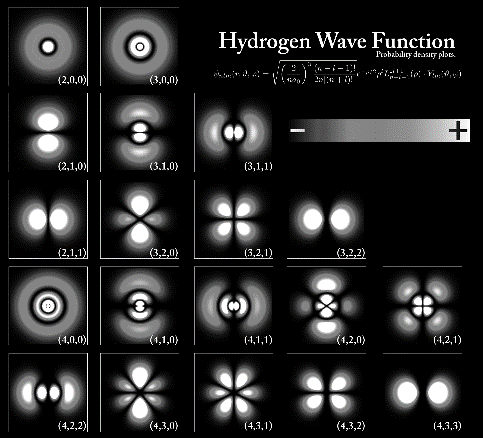
\includegraphics[width=\linewidth, center]{wave-function.png}
\label{fig:wave-function}
\end{figure}
有個比較好理解,但是被過度簡化的例子-環形駐波

把電子想成繞著核運行的波,我們剛剛有學到,最基本的穩定波是駐波,所以會穩定下來的電子波就是環形的駐波,而且駐波也有量子化的影子,故許多人講解波耳行星模型常引用這個說法,但其實波耳原本的解釋沒有提到。
\begin{figure}[H]
\centering
\graphicspath{{physics/}}
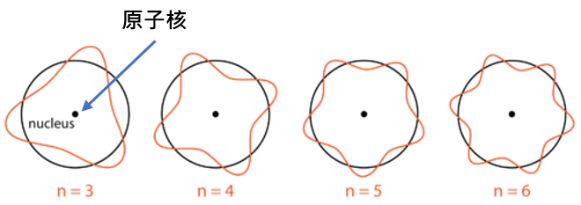
\includegraphics[width=\linewidth, center]{standing-wave.png}
\label{fig:standing-wave}
\end{figure}
\end{tcolorbox}
\section{奇怪的單粒子雙狹縫干涉}
\noindent
\begin{minipage}{0.7\linewidth}
\setlength{\parindent}{2em}
\setlength{\parskip}{1em}
\renewcommand{\baselinestretch}{1.1}
讓我們在來做個思維實驗,在自己腦海裡想像一個雙狹縫,我們再進行一次楊格的光的雙狹縫干涉實驗,但這一次,我們已經知道,光波的最基本單位是光子,一個光子的能量非常小,這代表每個光子必須要決定要穿過的是左邊的還是右邊的狹縫,而且光子已經是最小單位了,不能再分裂成一半然後在縫的後面合成。一般來說,我們發出的光裡面會有非常多的光子,所以從直覺上來看,只要有兩個以上的光子,出現干涉的條紋應該很正常,各個光子分別穿過不同狹縫,穿過狹縫後在狹縫的後方干涉形成條紋。

但是,如果只有一個光子呢?我們把光源的放出光的功率壓到非常低(後來真的有人做到了),所以光變成不是一大坨的光子一起穿越狹縫,而是一個一個的漫漫發射,這樣應該不會干涉了吧?因為它們都是自己一顆過去的。一開始,後方的屏幕很正常的出現了許多被光子打到形成的光點,幾顆幾顆的慢慢出現,一開始看起來是隨機分布的,但當時間過去,光點越來越多,我們發現光點的分布居然還是像原本的干涉條紋一樣!光點最多的地方對應到原本干涉條紋上的亮紋,反之亦然。

這個現象也發生在其他粒子身上,比如電子,如果電子發射器一次只發射一個電子,出現的分布情形也和干涉條紋一致!更誇張的是連巴克球(碳60)這種大分子也會出現干涉條紋。
為什麼會這樣?答案沒有人知道,但有許多量子力學詮釋試圖解答。
\end{minipage}%
\hfill%
\begin{minipage}{0.2\textwidth}
\begin{figure}[H]
\centering
\graphicspath{{physics/}}
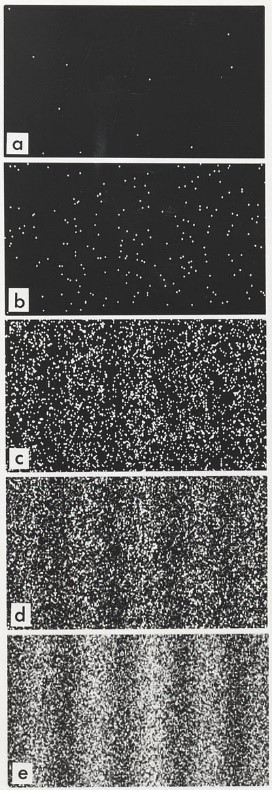
\includegraphics[width=\linewidth]{double-slit-exp.jpg}
\label{fig:double-slit-exp}
\end{figure}
\end{minipage}

\section{最多人相信的詮釋:哥本哈根詮釋}
由海森堡和玻恩等人的哥本哈根詮釋,因為它們都是哥本哈根大學研究量子力學的先驅,故得此名。

哥本哈根詮釋認為波函數沒有物理本質,是純粹的機率波,只有當他的位置\textbf{被觀察}的時候會出現\textbf{波函數崩塌},波函數本來是在空間中散播著,還沒被觀測時,他哪裡也不在,而且會出現波的干涉現象,但當你測量他的時候,他被迫要現身,這時候波函數會完全崩塌變成一個尖峰,這個尖峰就代表機率完全聚集在我們發現粒子的地方。而且重點是,這個波函數要崩塌在哪裡,完全取決於機率。

哥本哈根詮釋解決了我們的問題,卻也帶出了更多問題,像是為什麼觀測會讓波函數崩塌等等。其實,人們對量子力學還有更多詮釋,但其實不管它們怎麼解釋,都沒有人可以證明這些詮釋到底對不對,那麼,哪種詮釋比較好?其實沒人在乎,對於某些人,反正只要能算東西就好,他背後有什麼意義就留給想研究的人去研究吧,這也是\textbf{科學哲學}的研究對象之一,不過很多東西我也不懂,就沒有多做介紹了,只有簡報裡面稍微提到,想深入了解的話可以上網自己找資訊(感覺就沒人想知道)。

\section{不確定性原理}
由海森堡所提出的不確定性原理

\begin{center}
\noindent
{\Kai 一個運動粒子的位置和動量(質量乘以速度)不可被同時確定}
\end{center}

把這句話翻成更好理解的形式,他的意思是說,如果我們對粒子的位置進行測量,測量到的結果誤差越小,我們將無法確定他的動量是多少,反之亦然,如果測動量測得越準,我們就跟不能確定他的位置。
嗯,對於這段陳述,有些人可能會這樣理解。
當我們拿觀察電子等微觀粒子時,我們可能會需要拿光子去打他,但是測出電子的位置之後,光子可能會對他造成影響,造成動量的不確定。
\begin{figure}[H]
\centering
\graphicspath{{physics/}}
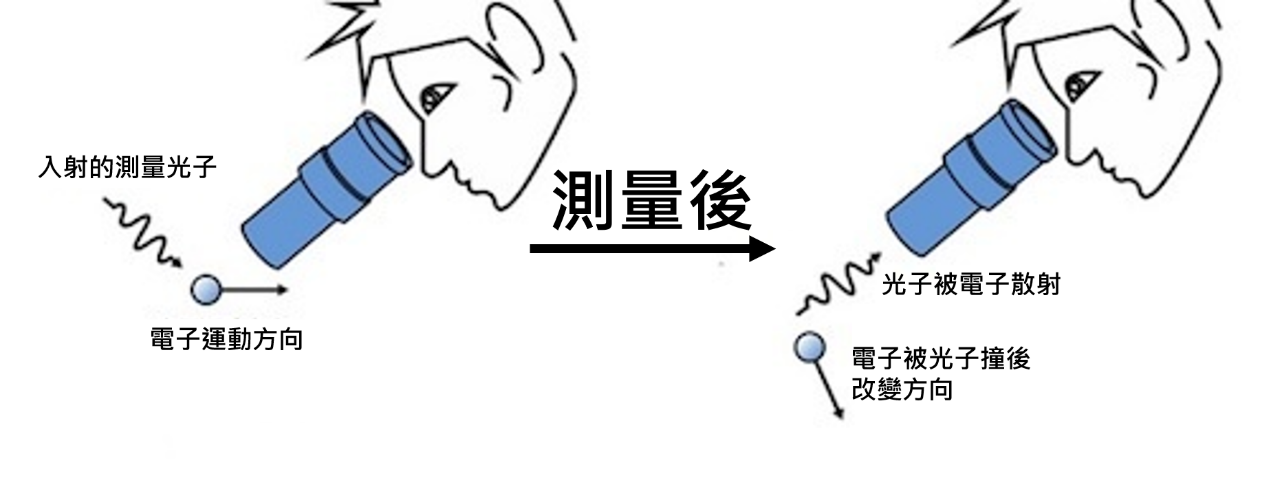
\includegraphics[width=\linewidth]{uncertainty-principle.png}
\label{fig:uncertainty-principle}
\end{figure}

照這個看法,不確定性是源於我們的測量儀器和技術不夠好?那如果我們真的找到一個更好的儀器或方法是不是就可以抹除不確定性?聽起來很合理?不過這其實是錯誤理解。

要進入量子力學的狀況,我們先來說說古典情況的不確定性。

假設你握著長繩的一端,有節奏的上下擺動產生一個波,如果有人問你,「這個波精確來說在哪裡?」,你沒辦法很好的回答,他分布在一個很寬的範圍,但如果有人問你「這個波的波長(頻率)是多少?」,你可以給出個合理的答案;反之,如果你快速的抖動一下繩子,將產生一個脈衝波,第一個問題(波在哪裡),就有很好的回答了,但第二個問題(波長是多少)卻又變得無法回答。這就是繩波的位置-頻率不確定性。
\begin{figure}[H]
\centering
\graphicspath{{physics/}}
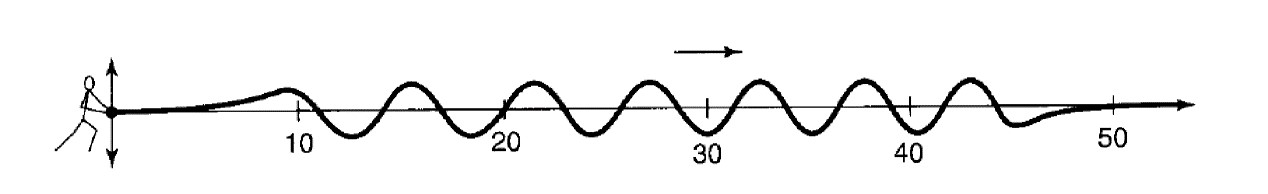
\includegraphics[width=\linewidth]{periodic-wave.jpg}
\caption{為週期波,頻率有很好的定義}
\label{fig:periodic-wave}
\end{figure}

\begin{figure}[H]
\centering
\graphicspath{{physics/}}
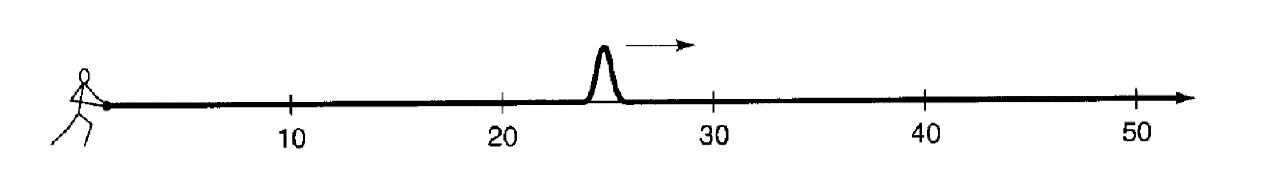
\includegraphics[width=\linewidth]{pulse-wave.jpg}
\caption{為為脈衝波,位置有很好的定義}
\label{fig:pulse-wave}
\end{figure}
回到量子的情況,德布羅意的物質波理論又說粒子的動量和波函數的頻率有關,所以古典的位置-頻率不確定性到量子世界中就變成位置-動量的不確定性。後人算出位置與動量的誤差滿足的關係(怎麼算出的又是另一個故事了)

$$
\Delta x \Delta p \geq \frac{h}{4 \pi}
$$

$\Delta x$表示位置的誤差,$\Delta p$表示動量的誤差,$h$表示普朗克常數,$\pi$是圓周率,你不必知道右邊的分數怎麼來的,你只要知道右邊的數非常小就好,所以當$\Delta x$越來越少,逼近於零,也就是位置的誤差越小,測量越精準,$\Delta p$就會暴增直到無限大,反之亦然。在巨觀的情況下,這個誤差小到可以忽略,但是對微觀物體來說就不能亂忽略了。

\section{結語} \label{justin-reflection}
看到這裡,相信許多人還是覺得頭昏腦脹(編按:我也是,排版好累,不過安磊真的很認真的在打這一章喔),但量子發展的一路走來是不可能用這堂課簡單帶過的!還有許多科學家的成就和發現都被省略了,以上都只是帶領你走馬看花,看見量子物理的奇妙之處,如果你瞥見了你中意的那朵花,那麼我的任務就達到了-「科學推廣」,接下來你要做甚麼都是你的事,你願不願意回去,自己踏過一遍量子的道路,拿著放大鏡好好的端詳那朵花;抑或是你認為物理和數學太難,不想深入研究,你們只要知道,眼前的這本講義,拿著這個講義的手,還有,你,都是很多的電子機率波在原子核周圍分布然後交互作用而已,卻能組合成這個複雜的世界,這也是他難以研究的原因,要是他好懂的話,可能我們就不存在了!
	
也請將要深入學習科學的同學謹記,我們不能讓每個人都參與科學研究的工作,但是其他人有權利知道這些研究的內容,請不要藏私,多和身邊對科學有誤解的人心平氣和的解釋而不是惱怒的否定。當你探索的越深,你一定會發現自己的無知,希望你會將這些疑惑轉化為動力,繼續追問,繼續探索下去。

\section{附錄:馬克士威方程式概述} \label{maxwell}
為了滿足想了解這四條方程式的同學,再把這些方程式做進一步的介紹,當然,想要完全搞懂你數學要夠好,若你覺得你數學夠好,請參閱\textbf{林琦焜:圖解梯度散度與旋度}(右方QR Code),或是遇到問題也可以找我。(這四條方程式沒有證明,因為我們發現他成正比而已)

\subsection{第一條:高斯定律\texorpdfstring{$\nabla \cdot \mathbf{E}=\frac{\rho}{\varepsilon_{0}}$}{TEXT}}
其中E表示空間中某個位置電場,$\rho$表示空間中某個位置的電荷密度,而$\nabla \cdot \mathbf{E}$表示$\mathbf{E}$在空間中的發散程度,因為電場是向量,你可以把他理解成\textbf{電場線},所以這條式子表示空間中某點電場線的發散程度,正比於空間中某點的電荷密度。事實上,將此式在球體區域積分後得到
$$
\int_{V} \nabla \cdot \mathbf{E} \mathrm{d} V=\int_{S} \mathbf{E} \cdot d \mathbf{A}=\frac{1}{\varepsilon_{0}} \int_{V} \rho \mathrm{d} V \Rightarrow 4 \pi r^{2} \mathbf{E}=\frac{Q_{e n c}}{\varepsilon_{0}}
$$

其實這就是庫倫定律,如果你努力的看還是不懂,我很難過,如果你看懂了,我更難過,我學了好久阿!!!

\subsection{第二條:高斯磁定律\texorpdfstring{$\nabla \cdot \mathbf{B}=0$}{TEXT}}
這條式子就像上面一樣,但是他永遠等於零,我們再回到第一條,如果有電荷密度,那麼電場的發散程度就不是零,如果沒有,那麼電場的發散程度就是零,所以這條式子就告訴我們,\textbf{沒有磁荷存在}(如果你能找到磁荷,恭喜你得諾貝爾獎)

\subsection{第三條:法拉第電磁感應定律\texorpdfstring{$\nabla \times \mathbf{E}=-\frac{\partial \mathbf{B}}{\partial t}$}{TEXT}}
積分後能夠把他變成一個比較好理解的形式
$$
\mathcal{E}=-\frac{d \Phi_{\mathrm{B}}}{d t}
$$

其中$\mathcal{E}$表示電動勢(就是電池的電壓), $\Phi_{\mathbf{B}}$表示磁通量,即磁場$\times$面積,所以這條式子就代表如果磁通量發生變化,就會產生一個電動勢。

\subsection{第四條:安培定律\texorpdfstring{$\nabla \times \mathbf{B}=\mu_{0} \mathbf{J}+\mu_{0} \varepsilon_{0} \frac{\partial \mathbf{E}}{\partial t}$}{TEXT}}
我們先忽略右邊的$\mu_{0} \varepsilon_{0} \frac{\partial \mathbf{E}}{\partial t}$的這一項,右邊的$\mathbf{J}$代表電流密度,左邊的$\nabla \times \mathbf{B}$表示磁場在某點旋轉的程度,所以這條式子代表若在這一點有電流,就會產生旋轉的磁場。

唬爛就到這裡,感覺有講跟沒有講一樣。

\section{講師介紹}
\begin{itemize}
\item 姓名:丁安磊
\item 性別:男
\item 特色:長得十分高壯,但不會打球(編按:聽說有時候體育課會偷跑回教室,根據本人說法是量子穿隧效應所導致)、十分有研究精神,常會研究某一些生物動力學問題到凌晨3、4點(編按:導致熊熊約講師出來看書時,約9點,講師通常都12點才來,抑或是直接不來了QQ)、對科技有興趣,有全班最酷的筆電Microsoft Surface、物理非常電、因為一直沒交講義,使熊熊十分惱怒。
\item 名言:喔我想到了,我們可以在科推加這個,一定超酷。(這些行為差點導致開天窗)
\end{itemize}
